%!TEX root = ../thesis.tex
\newchap{Statistical methods}\label{sec:STAT}
\minitoc
\section{Neural networks}
\subsection{Attention mechanism}

\section{Signal extraction}
The signal extraction procedure relies on a fit of a binned distribution.
The corresponding likelihood is a product of Poisson distributions, one for each bin, that contains the parameter of interest (POI) to fit.\\
Given C channels, each that contains $P_c$ processes, represented with histograms with $B_c$ bins, once we have the signal and the background MC prediction $s_{cb}$, $b_{cb}$, and the bin content $n_{cb}$ \footnote{Index $c$ stands for "channel", p for "process", b for "bin"}, the likelihood is \ADDREF higgspaper
\begin{equation}
    \mathcal{L}(\mu)=\prod_c^C \prod_b^{B_c} \frac{(\mu s_{cb}+b_{cb})^{n_{cb}}}{n_{cb}!} e^{-(\mu s_{cb}+b_{cb})}
\end{equation}
In this case, the POI is the signal strength $\mu$, that is estimated by finding the value that maximizes the likelihood, using the MIGRAD algorithm \ADDREF.
\begin{equation*}
    \hat{\mu}=argmax_\mu \mathcal{L}(\mu)
\end{equation*}

\subsection{Systematic uncertainties}
To incorporate in the model all the relevant uncertainties (\ie luminosity and rate uncertainties, uncertainties related to the detector resolution, etc.) we add to the likelihood the so-called nuisance parameters $\vec{\theta}$.\\
The likelihood becomes \cite{Conway2011IncorporatingSpectra}
\begin{equation}\label{eq:likelihood}
    \mathcal{L}(\mu,\vec{\theta})=\prod_c^C \prod_b^{B_c} Poiss \big( n_{cb}| \lambda_{cb}(\mu,\vec{\theta}) \big)  \prod_k  \pi_{k}(\theta_k)
\end{equation}
where $\pi_{k}$ is the prior probability distribution of the nuisance $\theta_k$.\\
The expectation value $\lambda_{cb}$ of the Poisson distribution now depends on the nuisance parameters that can be classified into normalization nuisances, shape nuisances and statistical nuisances.
\begin{equation}\label{eq:lambda}
     \lambda_{cb}( \mu,\vec{\theta})=\sum_p^{P_c}M_{cp}(\mu) N_{cp}(\vec{\theta}_n)y_{cpb}(\vec{\theta}_s)+E_{cb}(\vec{\theta}_{MC})
\end{equation}
The term $M_{cp}(\mu)$ is the physical model that contains the POI to fit, $N_{cp}(\vec{\theta_n})$ contains the factors relative to normalization nuisances, $y_{cpb}(\vec{\theta}_s)$ is the predicted content of each bin (that depends on shape nuisance parameters) and $E_{cpb}(\vec{\theta}_{MC})$ represents bin per bin the statistical error of the Monte Carlo predictions.\\
In the absence of systematic uncertainties, we have $N_{cp}=1$ and $E_{cb}=0 \quad \forall c,p,b$ and
$M_{cp}=\mu$ if $p$ is a signal process, otherwise $M_{cp}=1$; while $y_{cpb}$ is just the predicted bin content for each process.\\
All the nuisance parameters $\theta_k$ are defined in units of standard deviations\footnote{it means that $\theta=\pm 1$ correspond to a $\pm 1 \sigma$ variation.}.\\
Given that we know that we know the central values and the standard deviations of all the variations, following the maximum entropy principle \ADDREF, we can use the normal distribution as a prior for all the nuisance parameters
\begin{equation}
    \pi_k(\theta_k)=\mathcal{N}\left(\theta_k|0,1\right)=\frac{1}{\sqrt{2\pi}}e^{-\frac{\theta_k^2}{2}}
\end{equation}
Describing in details all the types of nuisances:
\begin{itemize}
    \item \textbf{Normalization nuisances} are multiplicative corrections that affect the normalization of one process (\eg the cross-section uncertainties) or of all processes (\eg the luminosity uncertainties).\\
    This type of uncertainty does not change the shape of the histogram but changes the number of expected events.\\
    In $\lambda_{cb}$ [eq. \ref{eq:lambda}], they are represented by the term
    \begin{equation}
        N_{cp}\left(\vec{\theta}_n\right)=k_{cp}^{\theta^{(n)}_k}
    \end{equation}
    where $k_{cp}$ the relative $+1 \sigma$ variation from the nominal event yield for the process $p$ in the channel $c$ estimated through theory calculation of external measurements, while $\theta_{k}$ is the relative normalization nuisance parameter.\\
    \item \textbf{Shape nuisances}: Shape changing nuisances are produced by uncertainties
    that cause a different variation of event yields for each different bin.\\
    The model parameters are varied of $\pm 1 \sigma$ around their central value, creating an “Up” and a “Down” variation.\\
    The bin content $y_{cpb}$ has to be modified by multiplying a continuous and differentiable function of $\vec{\theta}_{s}$, so, given $\delta_b^\pm$ the differences between the $\pm 1 \sigma$ bin content variations of the bin and the nominal one, the up and down variations are interpolated with a spline in a procedure called "vertical morphing" \ADDREF
    \begin{equation}
    f_b\left(\theta_k^{(s)}\right)=
        \begin{cases}
            {\frac{1}{2}}\left((\delta_b^{+}-\delta_b^{-})\theta_k+{\frac{1}{8}}(\delta_b^{+}+\delta_b^{-})(3\theta_k^{6}-10\theta_k^{4}+15\theta_k^{2})\right) & \text{for } |\theta_k|\leq 1\\
            \theta_k \delta^+ & \text{for } \theta_k>1\\
            -\theta_k \delta^{-} & \text{for } \theta_k<-1
        \end{cases}
    \end{equation}
    The term $y_{cpb}(\vec{\theta}_s)$ is then defined as 
    \begin{equation}
        y_{cpb}(\theta_s)=max\left(0,y_{cpb}+\sum_k f_{cpb}\left(\theta_k^{(s)} \right)\right)
    \end{equation}
    In this way we can clip $y_{cpb}$ to 0 preventing the height of the bin to being negative.\\
    The vertical morphing procedure is shown and described in details in \Fig{fig:morphing}

    \begin{figure}[h!]
        \centering
        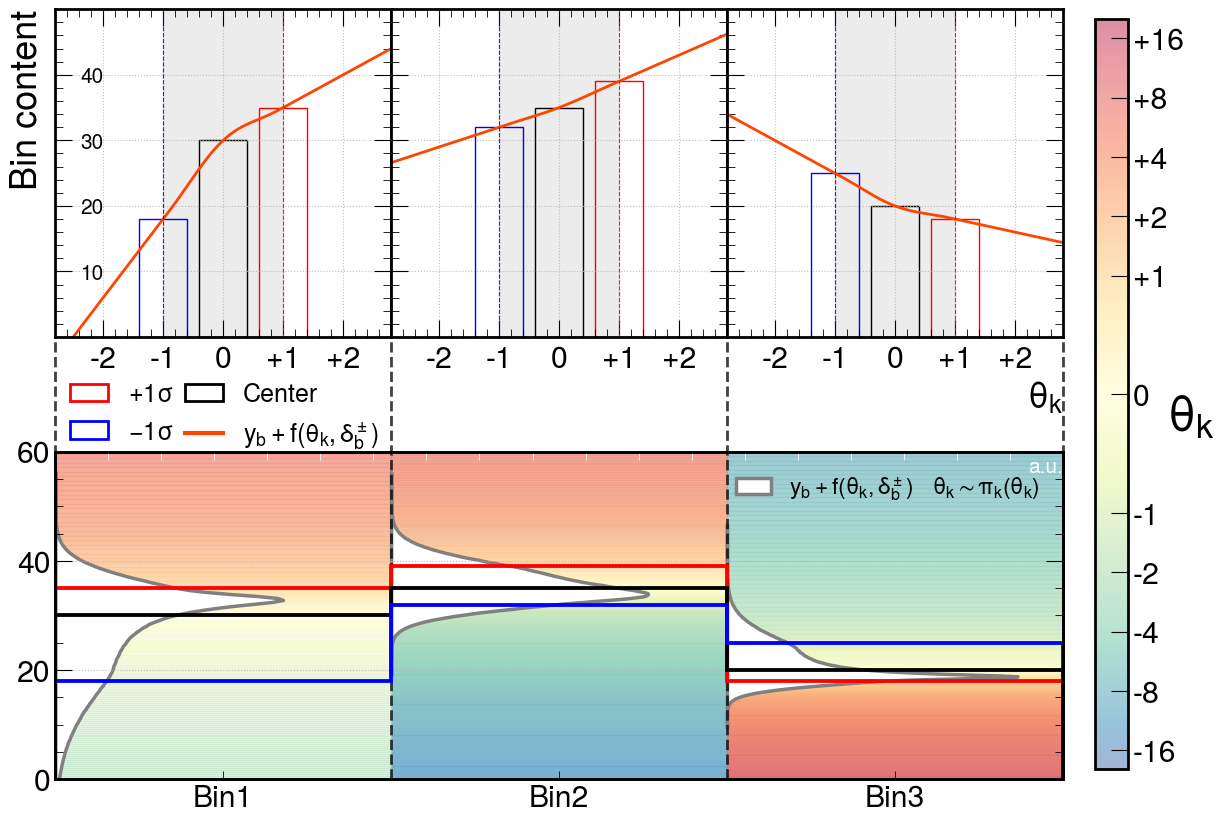
\includegraphics[width=\linewidth]{fig//chap05-stats/morphing.png}
        \caption{In the lower panel is represented an example of a histogram with 3 bins. The black line represents the histogram, the blue and the red lines represent the $\pm 1 \sigma$ shape variations.
        In the top panel, each bin is represented with its $\pm 1 \sigma$ variations and, on top of them, the $y_b+f(\theta_k,\delta_b^\pm)$ interpolation is shown with a red line. In the background of the lower panel, a color map shows, for each value of the bin height, the corresponding value of the nuisance parameter $\theta_k$, while the rotated vertical white shadow represents, for each bin, the probability distribution in arbitrary units of the expectation value of the Poisson distribution $\lambda_b=y_b+f(\theta_k,\delta_b^\pm)$ drawing $\theta_k$ from the normal prior.}
        \label{fig:morphing}
    \end{figure}


    
    \item \textbf{MC statistical nuisances}: The MC events used to predict the expected signal and background yield in each bin are limited.\\
    To model the statistical MC uncertainties, we could add a nuisance parameter per bin per process, following the Barlow-Beeston approach \ADDREF.\\
    But, if we have enough statistics in each bin, we can just use a nuisance parameter per bin that scales the sum of the processes yield, following the Barlow-Beeston lite approach \ADDREF.\\
    The term $E_{cb}$ in $\lambda_{bc}$ is the term related to the statistical uncertainties is
    \begin{equation}
        E_{cb}(\vec{\theta}_{MC})=\theta_b\left(\sum_p \left(e_{cpb}N_{cp}(\vec{\theta}_n)M_{cp}(\mu)\right)^2 \right)^{1/2}
    \end{equation}
    where $N_{cp}$ and $M_{cp}$ are the normalization factor and the physical model defined before.
    $e_{cpb}$ is the Poissonian standard deviation of b-th bin in the process p. Considering that the $\sigma_{Poiss}=\sqrt{N}$ and that the bin height has to be rescaled to match the expected number of observed events, $e_{cpb}$ is
    \begin{equation}
        e_{cpb}=\frac{\mathcal{L_I} \sigma_p \epsilon_{cp}}{\sqrt{N^{MC}_{cpb}}}
    \end{equation}
    where $\mathcal{L_I}$ is the integrated luminosity, $\sigma_p$ the cross-section of the process p, $\epsilon_{cp}$ the fraction of events of the process p that pass the preselection of the channel c, and $N_{cpb}^{MC}$ is the total number of MC events in the bin b after the preselection.\\
    The term $E_{cb}$ scales, linearly with the nuisance parameter, the event yield of the bin with the root square sum of the Poisson uncertainties of each process.\\
    

\end{itemize}
To improve the numerical stability, the software implementation exploits the negative log likelihood $\textit{NLL}=-\log{\mathcal{L}}$ instead of the likelihood in the form of the \Eq{eq:likelihood}  

 
\subsection{Profile Likelihood}

\subsection{Asimov dataset}

